\subsection{The LTCC Window}

The LTCC windows that covers the upstream and downstream open frame of the box is a composite of tedlar/mylar/tedlar, see \F{windowDesign}. The tedlar
material provides light tightness, while the mylar adds the necessary material strength necessary to withstand the gas pressure.

\begin{figure}
	\centering
	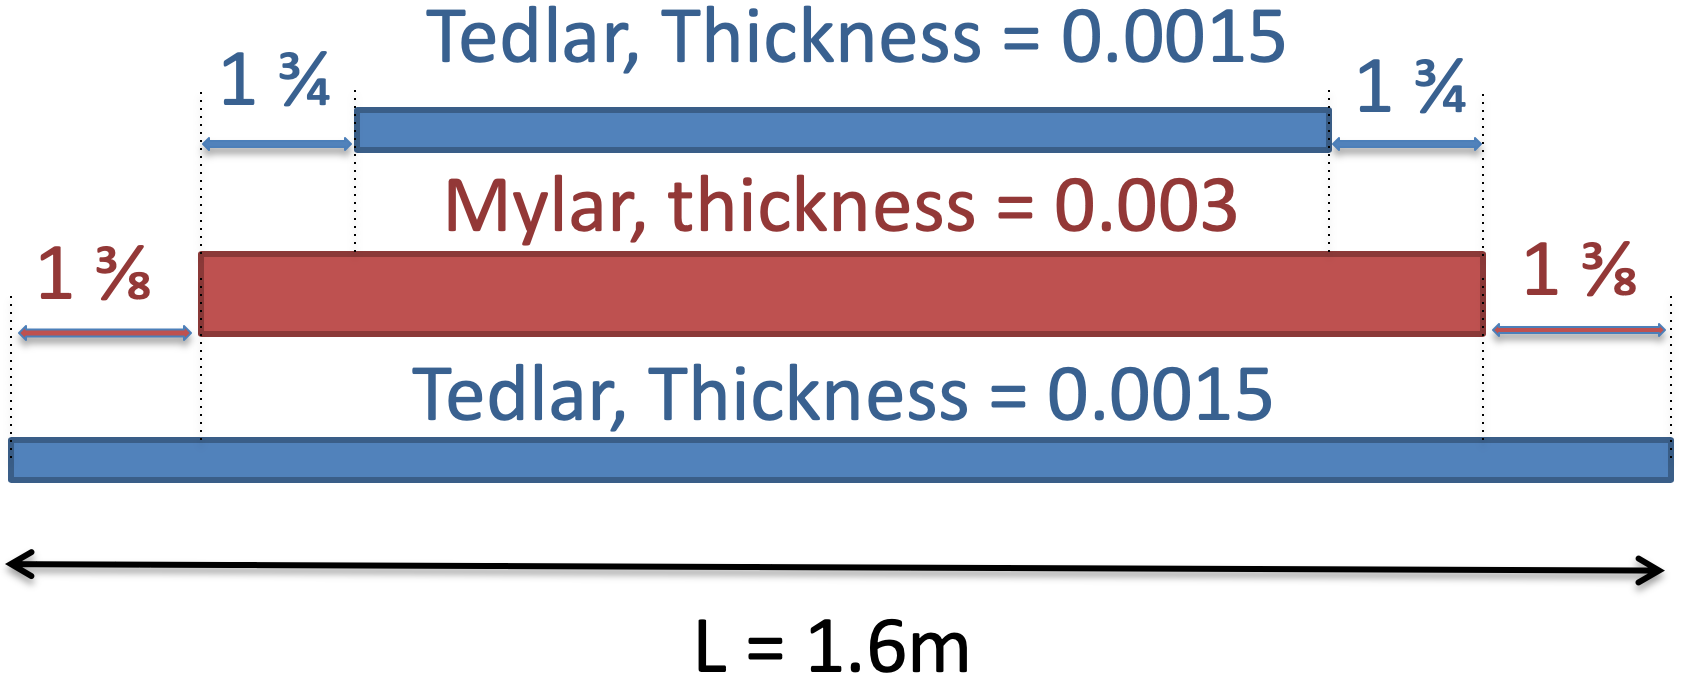
\includegraphics[width=1.0\columnwidth,keepaspectratio]{img/windowDesign.png}
	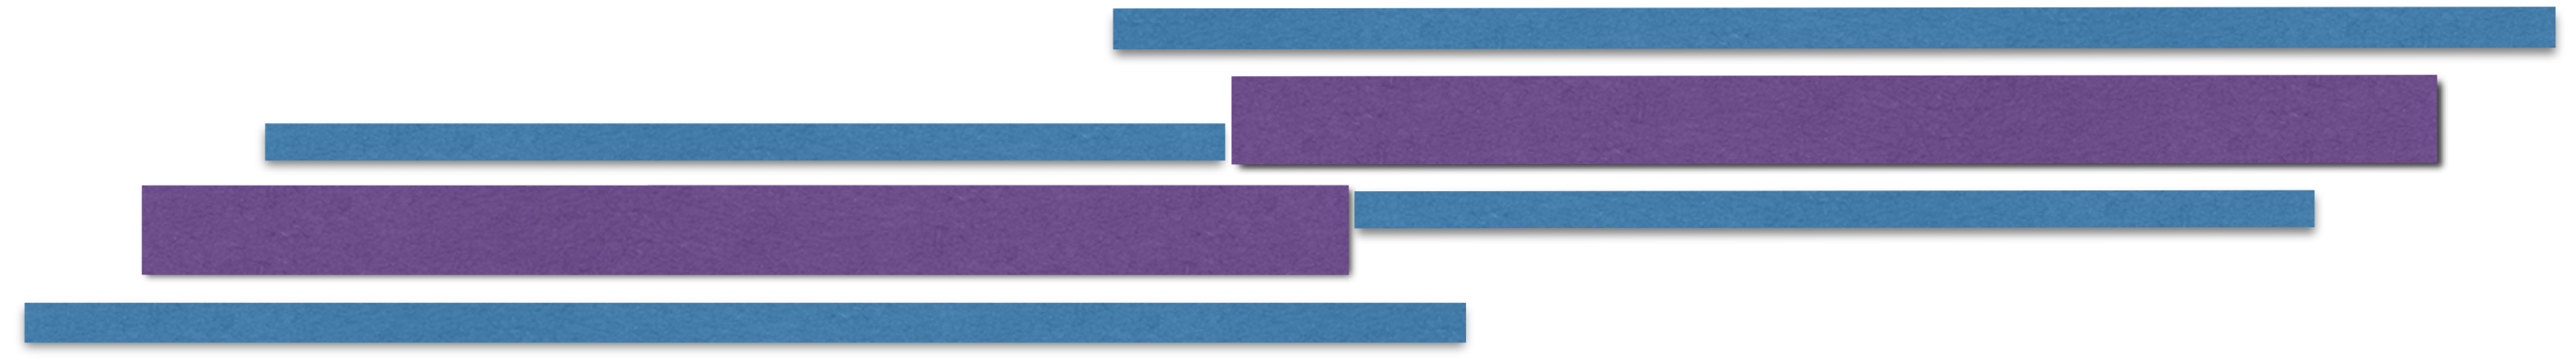
\includegraphics[width=1.0\columnwidth,keepaspectratio]{img/windowSeaming.png}
\caption{Top: the design of the window tedlar/mylar/tedlar sandwich. ML is 1.6m. The pyramid design allowed for the seaming shown at the bottom.
			Bottom: the seaming design involves gluing mylar to mylar to ensure that the window stress is transmitted entirely to the mylar. }
	\label{fig:windowDesign}
\end{figure}


The window was fabricated in two steps:

\begin{enumerate}
	\item lamination of tedlar/mylar/tedlar rolls 1.6m  wide
	\item seaming of the laminated strips into 4.8mx4.8m window
\end{enumerate}

The lamination of 400 yards of the composite material has been performed at Madico \cite{madico}.

\subsubsection{Windows seaming and tests}


The installation of the window onto the box is achieved through glue-ing the window on the box sides.


\begin{figure}
	\centering
	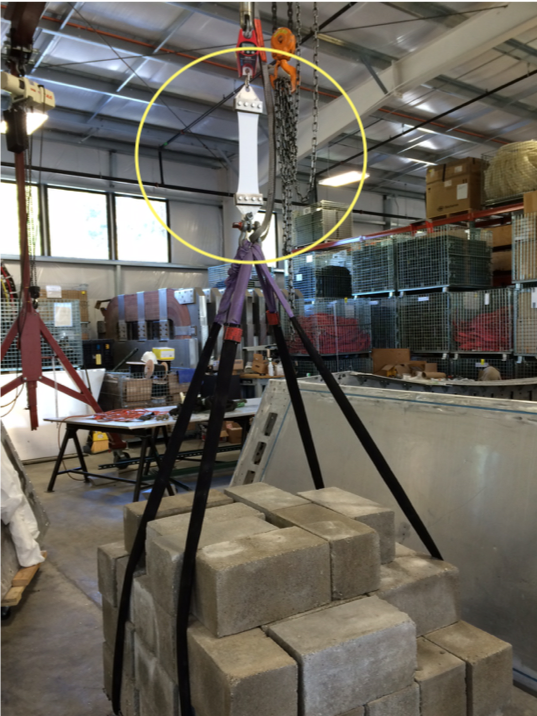
\includegraphics[width=1.0\columnwidth,keepaspectratio]{img/windowTest.png}
	\caption{The window was tested with up to 388 lbs of load. No significant damage was observed until rupture, which occured at a load of 388 lbs,
			   corresponding to about 15,000 psi of stress on the window, about a factor of 10 higher than the stress during normal operations of the detector.}
	\label{fig:windowTest}
\end{figure}



\subsubsection{Windows installation}

\begin{figure}
	\centering
	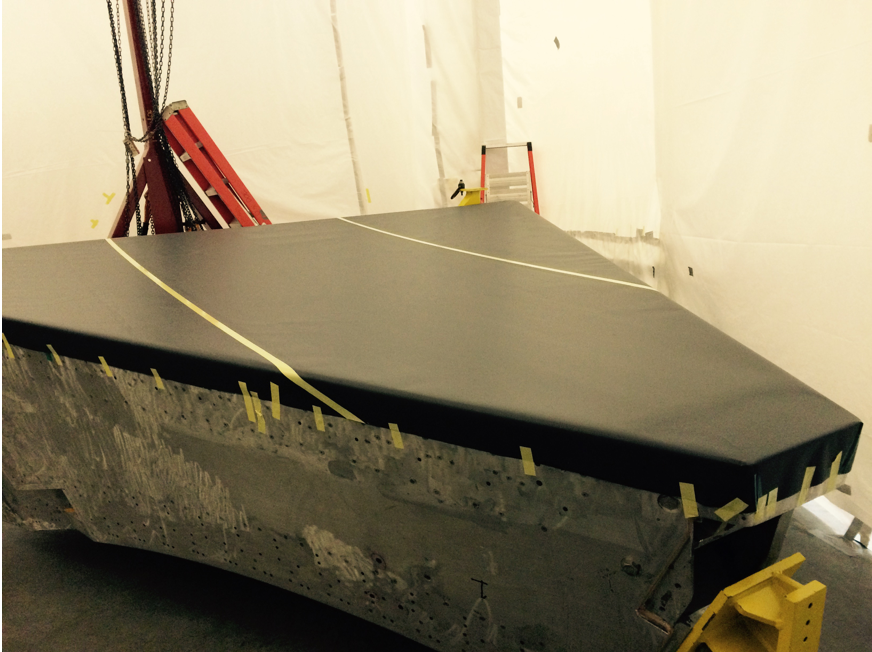
\includegraphics[width=1.0\columnwidth,keepaspectratio]{img/upstreamWindow.png}
	\caption{Top view of the back-wall of the LTCC. A stainless steel bar encapsulate a sandwich wall of aluminum and foam. On the left and right side
				 of the frame a new patch panel allow for 3 hermetical connectors (1 HV, 2 signals) from each PTM. }
	\label{fig:upstreamWindow}
\end{figure}




- Window to box glue + sealant

